% !TeX spellcheck = cs_CZ
%==================Kapitola: Teoretické základy radioelektroniky====================================
\setchaptertoc
\chapter{Teoretické základy radioelektroniky}\label{chap:ra_theory}

  %--------------- Úvod do šíření vln pro pozemní rádiové spoje ------------------------------------
  \section{Úvod do šíření vln pro pozemní rádiové spoje}
    \begin{example}
      Domácí meteostanice používá pro komunikaci s externím čidlem na měření vnější teploty 
      frekvenci \SI{433}{MHz}. Určete délku vln a rádiové pásmo do kterého použitá vlnová délka 
      patří.
      \newline\textbf{řešení:}
      \begin{equation}
        \lambda = c\cdot T = \frac{c}{f} = \frac{\num{300e6}}{\num{433e6}} = \SI{0.49}{\meter}
      \end{equation}
      Domácí meteostanice používá pro komunikaci s čidlem ultrakrátké vlny o vlnové délce 
      \SI{0.49}{\meter} 
    \end{example}
    
  %--------------- Základní klasifikace radioelektronických systémů --------------------------------
  \section{Základní klasifikace radioelektronických systémů}
    Pod pojmem systém \cite[s.~56]{ZaludRA} 

  \section{Dvojbrany v radioelektronice}
    Pod pojmem \emph{systém} se zde označuje elektrický obvod nebo soustava obvodů, které vytvářejí 
    alespoň jeden výstupní signál jako odezvu na alespoň jeden vstupní signál. Jednou z 
    nejdůležitějších tříd radioelektronických systémů jsou lineární systémy s časově invariantními 
    (neměnnými) parametry, které mají podobu \emph{n-branů}. Mezi nimi potom zaujímají významné 
    místo lineární dvojbrany a trojbrany, jejichž popisem a obecnými vlastnostmi se zabývá tato 
    kapitola. Připomeňme, že pro označení linearity a časové invariance se v teorii obvodů používá 
    zkratka \emph{LTI- (Linear Time Invariant)}, což nijak dále nezdůrazňujeme, nebo tato kapitola 
    je zaměřena právě jen na dvojbrany a trojbrany tohoto typu.
    
    V radioelektronice se často vyskytují dvojbrany a trojbrany, které přísně vzato lineární 
    nejsou, avšak jejich nelinearity jsou tak malé, že je lze v technické praxi zanedbat; do této 
    kategorie patří například všechny obvody s diodami a s tranzistory, pracujícími v režimu malých 
    signálů, kde jsou prakticky lineární a nelinearity se u nich začínají projevovat až při vyšších 
    úrovních signálů. Tyto dvojbrany a trojbrany, označované termínem kvazilineární (tedy téměř 
    lineární) Jsou rovněž zahrnuty do této kapitoly. Zvláštní pozornost je věnována zejména jejich 
    vlastnostem v hraniční oblasti mezi lineárním a nelineárním režimem, která je v 
    radioelektronice velmi důležitá.
    
    \subsection{Admitanční parametry a rozptylové parametry dvojbranů}
      Pod pojmem dvojbran (\emph{two-port}) se rozumí elektrický systém, který má jeden pár 
      vstupních svorek a jeden pár výstupních svorek, tedy jednu vstupní a jednu výstupní bránu 
      (dvojbran zřejmě představuje zvláštní třídu obecnějšího pojmu \emph{čtyřpól}, který má čtyři 
      nezávislé svorky). Linearizované přenosové vlastnosti dvojbranů je možné charakterizovat 
      pomocí jejich \textbf{admitančních} a \textbf{rozptylových parametrů}, kterým je dále 
      věnována náležitá pozornost \cite[s.~331]{ZaludRA}.
      
      Při definici \emph{admitančních parametrů} dvojbranů, nazývaných také parametry \(y\) 
      \emph{(Admittance Parameters)}, vyjdeme z obr. \ref{RA:fig_dvojbran01}. Zde je znázorněn 
      lineární časově invariantní dvojbran, který má na vstupu svorkové napětí a proud \(u_l\), 
      \(i_1\) a na výstupu \(u_2\), \(i_2\). K jeho vstupu je připojen generátor s vnitřní 
      admitancí \(Y_g\) a k výstupu zatěžovací admitance \(Y_z\). Admitanční parametry tohoto 
      dvojbranů jsou definovány relacemi
      \begin{align}
        i_1 &= y_{11}u_1 + y_{12}u_2   \\ 
        i_2 &= y_{21}u_1 + y_{22}u_2
      \end{align}
      
      \begin{figure}[ht!]
        \centering  
        \subcaptionbox{\label{RA:fig_dvojbran01}{\luafigure[0.45]{RA_dvojbran01.png}}
        \subcaptionbox{\label{RA:fig_dvojbran02}{\luafigure[0.45]{RA_dvojbran02.png}}
        \caption{Charakterizace dvojbranu: a) svorkovými napětími a proudy; 
                 b) dopadajícímí a odraženými napěťovými vlnami}\label{RA:fig_dvojbran}
      \end{figure}
      
      Z těchto vztahů vyplývá, že admitance \(y_{11}\) je rovna \emph{vstupní admitanci dvojbranu} 
      při jeho výstupu nakrátko (\(u_2=0\)), a podobně admitance \(y_{22}\) je \emph{výstupní 
      admitance} při vstupu nakrátko (\(u_1=0\)). Admitance \(y_{21}\), resp. \(y_{12}\) je potom 
      \emph{přenosová admitance} v předním nebo zpětném směru, při výstupu resp. vstupu nakrátko.
      
      Jak je patrné, parametry \(y\) jsou definovány při vstupu nebo výstupu nakrátko. Při jejich 
      měření však lze tuto podmínku splnit bez potíží jen při nižších kmitočtech, nepřesahujících 
      asi 300 MHz. Ve vyšších pásmech je možné vytvořit „zkrat“ např. vyladěným sériovým 
      rezonančním obvodem, nebo transformačním členem složeným z obvodů s rozloženými parametry, 
      což však příliš komplikuje měření (velké potíže vznikají zejména při návrhu širokopásmových 
      automatizovaných měřičů parametrů \(y\) s rozmítaným kmitočtem, které jsou v mikrovlnném 
      pásmu prakticky nerealizovatelné). Z tohoto, ale i z dalších důvodů byla během šedesátých let 
      propracována nová soustava parametrů označovaných jako parametry \(s\), nebo 
      \textbf{parametry rozptylové} (\emph{Scattering Parameters}). Definice rozptylových parametrů 
      dvojbranů vychází z obr. \ref{RA:fig_dvojbran02}. Zde je opět znázorněn lineární, časově 
      invariantní dvojbran, avšak jeho vlastnosti již nejsou charakterizovány svorkovými napětími a 
      proudy, ale \emph{normovanými dopadajícími napěťovými vlnami} \(a_1, a_2\) a \emph{odraženými 
      napěťovými vlnami} \(b_1, b_2\). Tyto vlny se vytvářejí na vstupním a na výstupním přenosovém 
      vedení o charakteristické impedanci \(Z_c\). Svorková napětí a proudy jsou vázány s 
      napěťovými vlnami jednoduchými vztahy
      \begin{align}\label{RA:eq_01}
      u_1 &= (a_1 + b_1)\cdot\sqrt{Z_c} \qquad i_1 = \frac{a_1-b_1}{\sqrt{Z_c}}   \\ 
      u_2 &= (a_2 + b_2)\cdot\sqrt{Z_c} \qquad i_1 = \frac{a_2-b_2}{\sqrt{Z_c}}
      \end{align}
      
      Naopak dopadající a odražené vlny jsou v závislosti na svorkových napětích a proudech určeny 
      vztahy
      \begin{align}\label{RA:eq_02}
      a_1 &= \frac{u_1 + i_1Z_c}{2\sqrt{Z_c}} \qquad b_1 = \frac{u_1 - i_1Z_c}{2\sqrt{Z_c}}   \\ 
      a_2 &= \frac{u_2 + i_2Z_c}{2\sqrt{Z_c}} \qquad b_1 = \frac{u_2 - i_2Z_c}{2\sqrt{Z_c}}
      \end{align}
      
      \emph{Charakteristická impedance} \(Z_c\), nazývaná v této souvislosti také \emph{impedancí 
      vztažnou (referenční)}, může obecně být komplexní veličinou; dále však předpokládejme, že je 
      reálná, stejná pro vstupní i výstupní bránu, s typickou hodnotou \(Z_c = \SI{50}{\ohm}\) (v 
      praxi se používají ještě impedance \SI{60}{\ohm} a \SI{75}{\ohm}). Vzájemnou závislost 
      dopadajících a odražených napěťových vln vyjadřují relace
      \begin{align}\label{RA:eq_03}
      b_1 &= s_{11}a_1 + s_{12}a_2   \\ 
      b_2 &= s_{21}a_1 + s_{22}a_2
      \end{align}
      které lze považovat za definiční vztahy rozptylových parametrů daného dvojbranu. Z nich se 
      snadno odvodí fyzikální význam jednotlivých parametrů:
      \begin{itemize}
        \item \textbf{vstupní napěťový činitel odrazu}, při výstupu zakončeném zátěží \(Z_z\), 
              přizpůsobenou k vztažné impedanci \(Z_c\)  (tj. \(Z_z = Z_c\) a tedy \(a_2 = 0\)):
              \begin{equation*}
                s_{11} = \left(\dfrac{b_1}{a_1}\right)_{a_2=0}
              \end{equation*}
        \item \textbf{výstupní napěťový činitel odrazu}, při vstupu zakončeném impedancí \(Z_g\), 
               přizpůsobenou k vztažné impedanci \(Z_c\) (tj. \(Z_g = Z_c\) a tedy \(a_1 = 0\)); 
              \begin{equation*}
                 s_{22} = \left(\dfrac{b_2}{a_2}\right)_{a_1=0}
              \end{equation*}
        \item \textbf{vložné napěťové zesílení v předním směru}, při výstupu zakončeném zátěží 
              \(Z_z\), přizpůsobenou k vztažné impedanci \(Z_c\) (tj. \(Z_z = Z_c\) a tedy \(a_2 = 
              0\));
              \begin{equation*}
                 s_{12} = \left(\dfrac{b_1}{a_2}\right)_{a_1=0}
              \end{equation*}
        \item \textbf{vložné napěťové zesílení v závěrném směru}, při vstupu zakončeném impedancí 
              \(Z_g\), přizpůsobenou k vztažné impedanci \(Z_c\) (tj.\(Z_g = Z_c\) a tedy \(a_1 = 
              0\)); \\
              \begin{equation*}
                 s_{12} = \left(\dfrac{b_1}{a_2}\right)_{a_1=0}
              \end{equation*}
      \end{itemize}
      
      Takto definované parametry \(s\) jsou závislé na impedanci \(Z_c\), proto jejich číselné 
      hodnoty je třeba vždy doplnit údajem o její hodnotě. Při grafickém znázornění se parametry 
      \(s_{11}\) a \(s_{22}\), představující \emph{činitele odrazu}, zakreslují obvykle do 
      příslušného rastru \emph{Smithova diagramu}; parametry \(s_{12}\) a \(s_{21}\) se potom 
      zobrazují do komplexní roviny, nejčastěji v polárním tvaru.
        
      V předchozích úvahách jsou rozptylové parametry definovány pomocí normovaných napěťových vln 
      \(a\), \(b\). Kvadráty modulů těchto vln \(a_2\) resp. \(b_2\) jsou rovny dopadajícím resp. 
      odraženým výkonům na vstupu a na výstupu dvojbranu. Proto se vlny \(a\), \(b\) označují také 
      jako výkonové vlny, ačkoliv přesněji vzato vyjadřují odmocniny z příslušných výkonů.
        
      Nehledě na to, že parametry \(y\) jsou definovány pomocí svorkových napětí a proudů a 
      parametry \(s\) pomocí dopadajících a odražených vln, existují mezi nimi vzájemné jednoznačné 
      vztahy. Tak např. parametr \(y_{11}\) definovaný pro \(u_2 = 0\), tj. pro 
      \(\dfrac{a_2}{b_2}=-1\), lze se zřetelem na převodní vztahy (\ref{RA:eq_01}), 
      (\ref{RA:eq_02}) vyjádřit ve tvaru
      \begin{equation}\label{RA:eq_04}
        y_{11} = \left(\frac{i_1}{u_1}\right)_{u_{22}} = \frac{a_1-b_1}{Z_c(a_1+b_1)} = 
                 \frac{1-\dfrac{b_1}{a_1}}{Z_c1+\left(\dfrac{b_1}{a_1}\right)} 
      \end{equation}
      Z definičních vztahů (\ref{RA:eq_03}) však plyne, že \(\frac{b_1}{a_1} = (\det s + s_{11})(1 
      + s_{22})\), kde \(\det s = s_{11}s_{22} -s_{21}s_{l2}\). Dosazením poslední relace do 
      (\ref{RA:eq_04}) se tedy získá převodní vztah
      \begin{equation}
        y_{11} = \frac{(1+s_{22})(1-s_{11})+s_{12}s_{21}}{(1+s_{11})(1+s_{22})-s_{12}s_{21}}
      \end{equation}
      
    \subsection{Vektorové měření impedance a přizpůsobení}
      \subsubsection{Činitel odrazu, přepočet na impedanci, poměr stojatého vlnění}
        Komplexní činitel odrazu \(\Gamma_L\) zátěže o impedanci \(Z_L\) připojené na konec 
        homogenního vedení o vlnové impedanci \(Z_0\) je v rovině připojení impedance \(Z_L\) 
        definován jako poměr fázoru harmonické napěťové vlny \(U^-\) na svorkách zátěže \(Z_L\), 
        která se od této zátěže odráží (odražená vlna), ku fázoru napěťové vlny \(U^+\) na svorkách 
        zátěže \(Z_L\), která na zátěži \(Z_L\) přichází po vedení (postupná vlna), tj.
        \begin{equation}\label{RA:eq_smith01}
          \Gamma_L = \frac{U^-}{U^+}
        \end{equation}
        Činitel odrazu je v této rovině funkcí pouze \(Z_0\) a \(Z_L\), přičemž obě tyto impedance 
        mohou být kmitočtově závislé (a také bývají, zejména \(Z_L\)).
  
        Mezi činitelem odrazu \(\Gamma_L\) a impedancemi \(Z_0\) a \(Z_L\) lze odvodit vztah
        \begin{equation}\label{RA:eq_smith02}
          \Gamma_L = \frac{Z_L-Z_0}{Z_L-Z_0}.
        \end{equation}    
        Pokud známe vlnovou impedanci vedení \(Z_0\) a činitel odrazu \(\Gamma_L\), lze ze vztahu 
        \ref{RA:eq_smith02} snadno vyjádřit zatěžovací impedanci \(Z_L\)
        \begin{equation}\label{RA:eq_smith03}
          Z_L = Z_0\frac{1+\Gamma_L}{1-\Gamma_L},
        \end{equation}    
  
        často udávaným parametrem popisujícím míru nepřizpůsobení je poměr stojatého vlnění - 
        \textbf{PSV} \emph{(Voltage Standing Wave Ratio - VSWR)}. Je definován jako poměr maximální 
        a minimální hodnoty amplitudy tzv. stojatého vlnění, které vzniká součtem postupné a 
        odražené vlny na vedení. Poměr stojatého vlnění lze vyjádřit taktéž pomocí vlnové impedance 
        vedení \(Z_0\) a zatěžovací impedance \(Z_L\), a tedy i pomocí činitele odrazu \(\Gamma_L\)
        \begin{equation}\label{RA:eq_smith04}
          PSV = \frac{U_{max}}{U_{min}} 
              = \frac{\abs{Z_L+Z_0} + \abs{Z_L-Z_0}}{\abs{Z_L+Z_0} - \abs{Z_L-Z_0}} 
              = \frac{1+\abs{\Gamma_L}}{1-\abs{\Gamma_L}}.
        \end{equation}
        Poslední výraz umožňuje odpoutat definici poměru stojatého vlnění od vedení a pracovat s 
        ním podobně jako s velikostí činitele odrazu \(\Gamma_L\).
      
      \subsubsection{Impedanční přizpůsobení pomocí obvodů se soustředěnými parametry}
        Přivádíme-li vysokofrekvenční signál z generátoru o vnitřní impedanci \(Z_G\) na zátěž o 
        impedanci \(Z_L\), je obvykle žádoucí dosažení stavu tzv. \emph{impedančního přizpůsobení}. 
        Přitom rozlišujeme dva typy impedančního přizpůsobení. Prvním je \emph{impedanční 
        přizpůsobení pro maximální přenos výkonu}, pro které platí
        \begin{equation}\label{RA:eq_smith05}
          Z_L = Z^*_G,
        \end{equation}  
        kde \(Z^*_G\) je komplexně sdružená hodnota k vnitřní impedanci generátoru \(Z_G\). V tomto 
        stavu obdržíme na zátěži \(Z_L\) největší činný výkon, jaký je generátor vůbec schopen do 
        nějaké zátěže dodat - tzv. \emph{dosažitelný výkon}.
  
        Druhým typem je \emph{bezodrazové impedanční přizpůsobení}, vhodné v případě, kdy na zátěž 
        \(Z_L\) přivádíme signál po vedení o vlnové impedanci \(Z_0\) nezanedbatelné délky vzhledem 
        k vlnové délce signálu. V tomto stavu platí
        \begin{equation}\label{RA:eq_smith06}
          Z_L = Z_0,
        \end{equation}  
        a jeho výhodou je, že při něm na konci vedení nedochází k odrazům, které by jinak mohly 
        kromě zhoršení účinnosti přenosu výkonu způsobit také degradaci kvality signálu (v případě 
        odrazů na obou koncích vedení, např. tzv. „duchy“ v televizním obrazu způsobené právě 
        nepřizpůsobeným anténním napáječem). Jelikož u většiny vedení máme v praxi téměř nulovou 
        imaginární část vlnové impedance \(Z_0\) (přesně nulovou mají bezeztrátová vedení), je 
        bezodrazové impedanční přizpůsobení obvykle současně přizpůsobením pro maximální přenos 
        výkonu (avšak pouze za předpokladu, že je provedeno na obou koncích vedení, tj. jak na 
        straně zátěže, tak na straně generátoru).
  
        V našem případě budeme bezodrazově přizpůsobovat určitou zatěžovací impedanci \(Z_L\) k 
        vedení o reálné vlnové impedanci \(Z_0 = \SI{50}{\ohm}\) (půjde tedy současně i o 
        přizpůsobení na maximální přenos výkonu). To znamená, že budeme navrhovat přizpůsobovací 
        obvod (viz obr. \ref{fyz:fig0_RA_smith01}), který zakončen na svém  výstupu impedancí 
        \(Z_L\) bude při daném kmitočtu vykazovat vstupní impedanci rovnou \(Z_0 = \SI{50}{\ohm}\).
        \begin{figure}[ht!] %\ref{fyz:fig0_RA_smith01} 
          \centering
          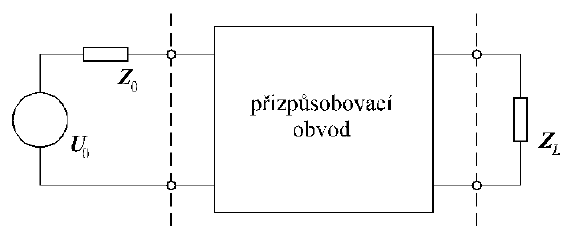
\includegraphics[width=0.5\linewidth]{RA_smith01.png}
          \caption{Umístění přizpůsobovacího obvodu mezi zátěží a zdrojem signálu (vedením)}
          \label{fyz:fig0_RA_smith01} 
        \end{figure}
        K tomuto účelu vystačíme s nejjednodušším typem zapojení, které umožňuje dosažení 
        přizpůsobení na jednom kmitočtu s tzv. \(\Gamma\text{-články}\). Jde o kaskádní řazení 
        dvojice reaktančních prvků, z nichž jeden je vždy v podélné a druhý v příčné větvi bez 
        ohledu na pořadí. V rezistivních obvodech totiž dochází ke ztrátám přenášeného výkonu, 
        zatímco obvody složené z reaktancí slibují (alespoň teoreticky) dosažení přizpůsobení beze 
        ztrát. Kombinací obou pořadí s typy reaktančních prvků (kondenzátor, cívka) dostáváme 
        celkem osm různých možností uspořádání \(\Gamma\text{-článků}\), přičemž volba konkrétní 
        struktury závisí především na hodnotě přizpůsobované impedance \(Z_L\). Obrázek 
        \ref{RA:fig_smith02}  ukazuje jednotlivé vhodné struktury v závislosti na umístění 
        impedance \(Z_L\) v impedančním Smithově diagramu v jedné z osmi oblastí \emph{A} až 
        \emph{H}, při aplikaci požadavku přesunu z bodu \(Z_L\) do bodu \(Z_0\) co nejkratší 
        cestou. Hlavní myšlenka zde spočívá v tom, že do bodu \(Z_0\) se lze dostat jedině pohybem 
        po kružnici jednotkové reálné části impedance (\(r = 1\)) nebo admitance (\(y = 1\)), a to 
        buď po směru nebo proti směru hodinových ručiček. To zajišťuje první prvek 
        \(\Gamma\text{-článku}\) - sériově nebo paralelně řazený induktor nebo kapacitor. Z toho 
        plynou čtyři varianty označené malými písmeny „\emph{a}“ až „\emph{d}“. Úkolem 
        druhého stupně je přesun z bodu \(Z_L\) na jednu (obvykle tu nejbližší) z obou zmíněných 
        kružnic opět sériově nebo paralelně řazeným induktorem nebo kapacitorem - odtud tedy osm 
        variant přizpůsobení v oblastech \emph{A} až \emph{D}. Způsob návrhu 
        \(\Gamma\text{-článku}\) pomocí Smithova diagramu nejlépe objasníme na číselném příkladu.
  
        \begin{figure}[ht!] %\ref{RA:fig_smith02} 
          \centering
          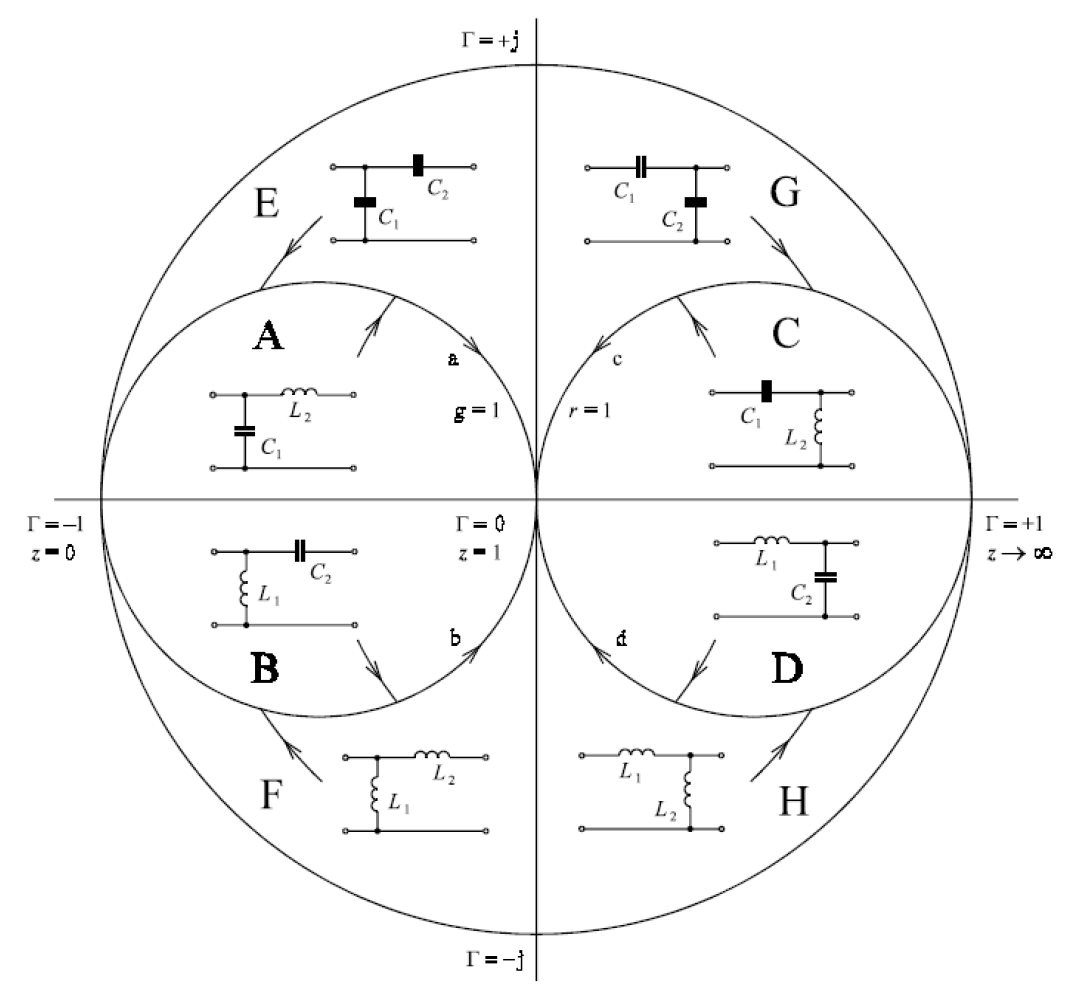
\includegraphics[width=\linewidth]{RA_smith02.png}
          \caption{Vhodné způsoby přesunu ve Smithově diagramu a odpovídající struktury  
          \(\Gamma\text{-článků}\)}
          \label{RA:fig_smith02} 
        \end{figure}
        %------------------------------------
          % !TeX spellcheck = cs_CZ
% RA_exam01.tex
\begin{example}
  Navrhněte graficko-početní metodou ve Smithově diagramu přizpůsobovací obvod pro 
  \(Z_L = \qty{30 - 65j}{\ohm}\) , \(Z_S = 50\)  a \(f = \qty{100}{\MHz}\).
  
  \textbf{Řešení:}
  Platí \(z_L = \dfrac{Z_L}{Z_S} = \num{0.6000 - 1.3000i}\), daný bod se tedy nachází ve 
  \textbf{4. kvadrantu}, \textbf{vně} kružnice konstantní reálné části impedance \(r = 
  1\). Proto volíme strukturu typu \(H\) viz. obr. \ref{RA:fig_smith02}. 
  \newline
  \begin{itemize}
    \item 1. krok: Začínáme v admitančních souřadnicích. Pro posun z bodu \(y_L = 
          \dfrac{1}{z_L} = \num{0.2927 + 0.6341i}\) nejkratší cestou na kružnici \(r = 1\), 
          tj. do bodu \(y_1 = \num{0.2927 + 0.4500i}\), musíme z admitance \(y_L\) ubrat 
          normovanou susceptanci \(\num{0.6341} - \num{0.4500} = \num{0.1841} = \Delta b = 
          \dfrac{\omega L_2}{Z_0}\). Paralelní indukčnost \(L_2\) tedy bude
          \MULTIPLY{2}{\numberPI}{\nmbrA}
          \MULTIPLY{\nmbrA}{100}{\nmbrB}
          \MULTIPLY{\nmbrB}{0.1841}{\nmbrC}
          \DIVIDE{50}{\nmbrC}{\nmbrD}
          \MULTIPLY{1000}{\nmbrD}{\nmbrE}
          \ROUND[2]{\nmbrE}{\sol}
          \begin{equation*}
            L_2 = \frac{Z_0}{\omega\abs{\Delta b}} = 
                  \frac{50}{2\cdot\pi\cdot\num{100e6}\cdot\num{0.1841}} = \qty{\sol}{\nano\henry}
          \end{equation*}
    
           {\centering   %\ref{RA:fig_RA_ADS_smith01} 
            \captionsetup{type=figure}
            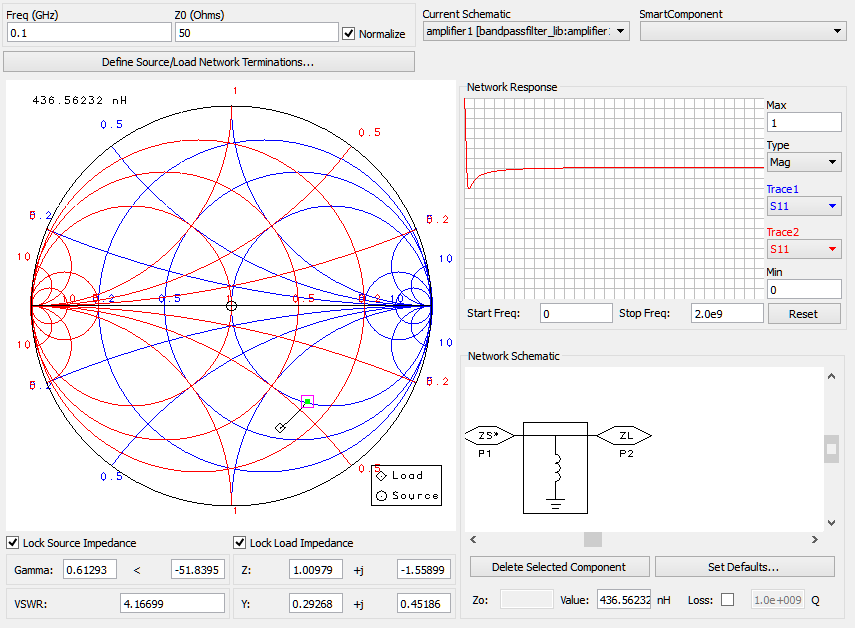
\includegraphics[width=0.8\linewidth]{ADS_smith01.png}
            \captionof{figure}{ADS Smith Chart tool: Přechod z bodu \(y_L \rightarrow y_1\)}
            \label{RA:fig_ADS_smith01} 
            \par}
          
    \item 2.krok: Pro posun z bodu \(z_1 = \dfrac{1}{y_1} = \num{1 - 1.5479i}\) do bodu 
          \(z_S = \num{1 + 0i}\) musíme k \(z_1\) přidat normovanou reaktanci \(1.5479 = \Delta 
          x = \frac{\omega L_2}{Z_0}\). Sériová indukčnost \(L_1\) tedy bude
          \MULTIPLY{2}{\numberPI}{\nmbrA}
          \MULTIPLY{\nmbrA}{100}{\nmbrB}
          \MULTIPLY{50}{1.5479}{\nmbrC}
          \DIVIDE{\nmbrC}{\nmbrB}{\nmbrD}
          \MULTIPLY{1000}{\nmbrD}{\nmbrE}
          \ROUND[2]{\nmbrE}{\sol}
          \begin{equation*}
            L_1 = \frac{\Delta x Z_0}{\omega} = 
                  \frac{\num{1.5479}\cdot\num{50}}{2\cdot\pi\cdot\num{100e6}} = 
                  \qty{\sol}{\nano\henry}
          \end{equation*}
           
           {\centering   %\ref{RA:fig_RA_ADS_smith02}
            \captionsetup{type=figure} 
            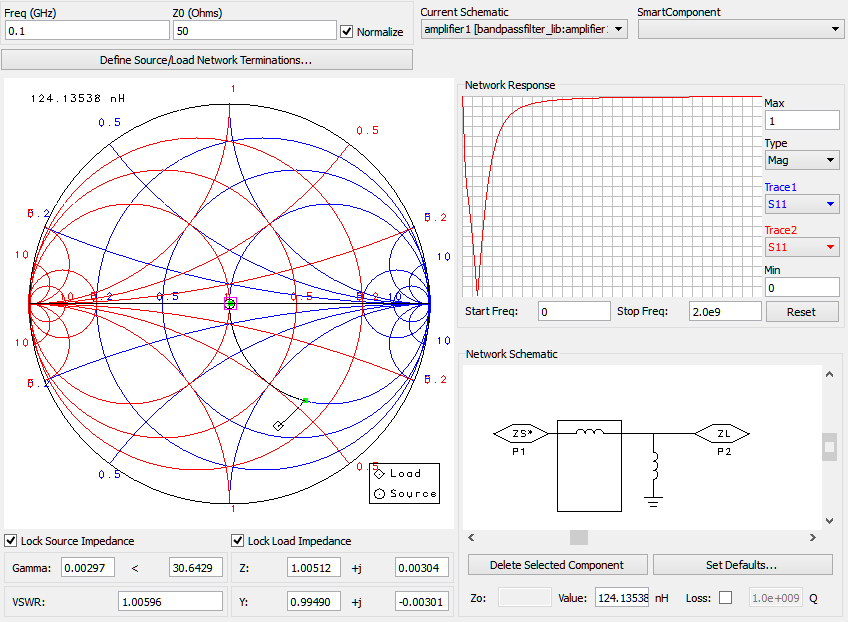
\includegraphics[width=0.8\linewidth]{ADS_smith02.png}
            \captionof{figure}{ADS Smith Chart tool: Přechod z bodu \(z_1 \rightarrow z_S\)}
            \label{RA:fig_ADS_smith02} 
            \par} 
  \end{itemize}
\end{example} 
        %------------------------------------
        Kromě přesunu nejkratší cestou přicházejí v úvahu ještě další varianty spojené s přechodem 
        do jiného segmentu. Např. pro \(Z_L\) v oblasti \(A\) lze použít též 
        \(\Gamma\text{-článek}\) typu \(B\); pro \(Z_L\) v oblasti \(E\) lze použít též typy \(B\), 
        \(D\) nebo \(G\) apod. Pro dosažení nejmenší kmitočtové závislosti lze však obvykle 
        doporučit pouze přesun nejkratší cestou.
  
      \subsubsection{Smithův diagram}
        \emph{Impedanční Smithův diagram} je soustava křivek (přesněji kružnic nebo jejich částí) 
        tvořených body normované impedance \(z\) s konstantní reálnou či imaginární částí 
        zakreslených v komplexní rovině činitele odrazu \(\Gamma\) definovaná konformním zobrazením
        \begin{equation}\label{RA:eq_smith07}
          \Gamma = \frac{z-1}{z+1}.
        \end{equation} 
  
        Každému bodu v Smithově diagramu odpovídá jedna hodnota normované impedance \(z = r + jx\), 
        a odnormované impedance \(Z = R+jX\). Otočením o 180°, popř. středovou souměrností, 
        získáme \emph{admitanční Smithův diagram} \(y = g + jb\), resp. \(Y = G + jB\). Kružnice 
        konstantních reálných částí se sbíhají v bodě \(1\) a mají středy na reálné ose. Kružnice 
        (části kružnic) konstantní imaginární části se taktéž sbíhají v bodě \(1\) a mají středy na 
        přímce Re [] = 1.
  
        Jelikož pro převod mezi poměrem stojatých vln a modulem činitele odrazu j􀀀j platí stejný 
        vztah jako mezi činitelem odrazu 􀀀 a normovanou impednací z, tj.
        \begin{equation}\label{RA:eq_smith08}
          \Gamma = \frac{z-1}{z+1} \qquad \Leftrightarrow 
          \abs{\Gamma} = \frac{\abs{PSV}-1}{z+\abs{PSV}}.
        \end{equation} 
        s rozdílem, že PSV je vždy reálné číslo větší nebo rovno jedné, lze PSV pro daný bod ve 
        Smithově diagramu určit z průsečíku kružnice se středem v bodě z = 0 a poloměrem j􀀀j a 
        části reálné osy normované impedance mezi body z = 1 a z ! 1.
        
      \subsubsection{Měření činitěle odrazu} 
        Abychom mohli měřit činitel odrazu podle definice (1), musíme mít možnost
        \begin{itemize}
          \item oddělit vlnu odraženou (U¡) od vlny dopadající (U+)
          \item měřit komplexní poměr fázorů napětí na příslušném kmitočtu.
        \end{itemize} 
        
        Splnění prvního požadavku nám zajišťuje tzv. směrový vazební člen (SVČ), splnění druhého 
        požadavku pak vektorový voltmetr. Celkové uspořádání měřicí sestavy využívající směrového 
        vazebního členu a vektorového voltmetru znázorňuje obr. 3. Harmonický signál potřebného 
        kmitočtu se rozděluje pomocí symetrického přizpůsobeného T-článku (splitteru) do tzv. 
        referenční a měřicí větve. Obě větve jsou zakončeny terminátory o impedanci rovné vlnové 
        impedanci Z0 vedení a konektorů, aby zde nedocházelo k nežádoucím odrazům a stojatému 
        vlnění. Ke snížení stojatého vlnění též přispívají pevné útlumové články v obou větvích 
        (20, 14 a 6 dB). Napětí v obou větvích jsou snímána sondami vektorového voltmetru 
        zasunutými do průchozích držáků. Měřená zátěž ZL je připojena na konec hlavního vedení 
        směrového vazebního členu SVč . Odražená vlna se potom vyvazuje na bránu 4 (přes vazbu K2 
        SVČ) a její amplituda a fáze je měřena sondou B vektorového voltmetru. Sonda A v referenční 
        větvi poskytuje fázovou referenci pro stanovení fáze činitele odrazu.
  
        Měření činitele odrazu probíhá ve dvou krocích:
        \begin{itemize}
          \item Nastavení amplitudové a fázové referenční hodnoty. Měřicí aparaturu je třeba 
          zkalibrovat tak, aby udávaný modul a fáze činitele odrazu pro nějakou zátěž, jejíž 
          činitel odrazu předem známe, této hodnotě přesně odpovídal. K tomuto účelu se obvykle 
          používá zkrat (Z = 0, 􀀀 = ¡1;0), ale v našem konkrétním případě se jako vhodnější ukazuje 
          otevřený konec vedení (Z ! 1, 􀀀 = +1;0), neboť naměřená odražená vlna při něm vykazuje o 
          něco větší amplitudu než při zakončení zkratem. Bránu 3 SVč (konec hlavního vedení) tedy 
          necháme nezakončenou a na generátoru nastavíme příslušný kmitočet f a vhodnou amplitudu 
          (zpravidla největší přípustnou, pro dobrý odstup signálu od šumu ve vektorovém 
          voltmetru). Amplitudu napětí naměřenou v této situaci sondou B uložíme na přístroji 
          BM553 jako referenční stlačením tlačítek <B>, <LEVEL REF STORE> a fázový rozdíl 'B ¡'A 
          uložíme jako referenční tlačítkem <',T REF STORE>. Aplikaci uložené amplitudové 
          referenční hodnoty poté aktivujeme tlačítkem <LIN REF>. Přístroj by měl zobrazovat 
          správnou hodnotu 􀀀 pro zakončení naprázdno, tj. modul 1;0 a fázi 0±.
  
          \item Vlastní měření činitele odrazu 􀀀. Na bránu 3 směrového vazebního členu připojíme 
          měřenou zátěž. Bylo-li provedeno nastavení podle předchozího bodu, bude již přístroj 
          ukazovat správnou hodnotu činitele odrazu 􀀀 v polárních souřadnicích.   
        \end{itemize}
        
        Z uspořádání měřicího systému je zřejmé, že při měření činitele odrazu na více kmitočtech 
        je třeba po každé změně kmitočtu signálu celý první krok postupu zopakovat.
  
      \subsubsection{Směrový vazební člen}     
        Směrový vazební člen (SVČ, též směrová vazební odbočka, směrová vazební odbočnice, směrová 
        vazba) je vysokofrekvenční čtyřbran umožňující oddělení a měření složek signálu, které se 
        šíří po vedení pouze jedním směrem. Mezi jeho četné aplikace patří měření činitele odrazu, 
        oddělení signálního generátoru od měřicích obvodů, rozdělení výkonu a připojení dalších 
        přístrojů (vlnoměrů, analyzátorů, wattmetrů apod.).
  
        Princip SVČ je založen na vlastnostech obvodů s rozprostřenými parametry a jeho vnější 
        funkce je patrná z obrázku 4. Dva úseky vedení ‚- hlavní (zakončené branami 1 a 3) a 
        vedlejší/vazební (mezi branami 2 a 4) ‚- jsou spojeny tak, aby mezi nimi vznikla vazba. 
        Tato vazba způsobuje, že se signál zavedený na bránu 1 hlavního vedení rozdělí v určitém 
        poměru na dvě vzájemně fázově posunuté složky. Jedna složka vystupuje na bráně 3 a druhá 
        buď na bráně 2, přičemž brána 4 je dokonale izolována (protisměrný SVČ ), nebo na bráně 4, 
        přičemž brána 2 je izolována (souměrný SVČ ). Zmíněná vazba je reciprocitní a vykazuje 
        obdobné chování i ze směru od vedlejšího vedení k hlavnímu.      
  
        \begin{figure}\ref{fyz:fig0_RA_smith03} 
          \centering
          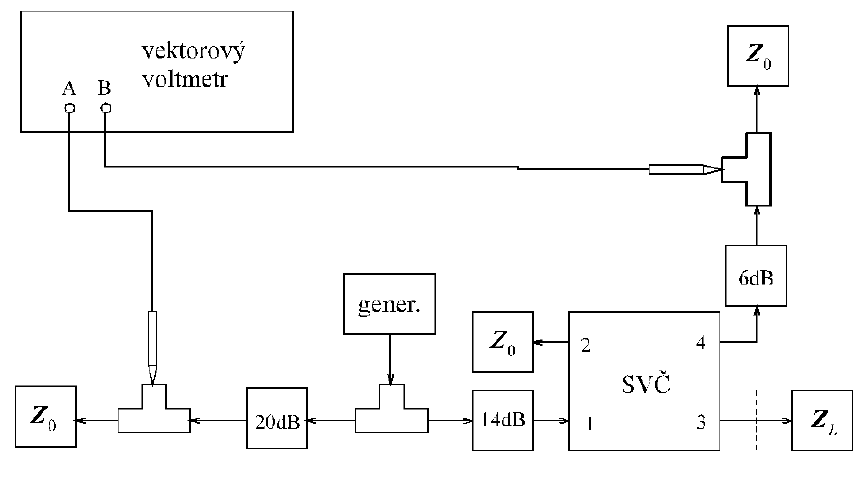
\includegraphics[width=\linewidth]{RA_smith03.png}
          \caption{Směrový vazební člen jako čtyřbran}
          \label{fyz:fig0_RA_smith03} 
        \end{figure}
  
        SVČ lze popsat maticí rozptylových parametrů o rozměru 4 Q 4, kde parametry skk na hlavní 
        diagonále jsou činitele odrazu na jednotlivých branách, ostatní parametry jsou činitele 
        přenosu mezi branami. U ideálního protisměrného (obr. 4) SVč jsou všechny činitele odrazu 
        rovny nule, přenos z brány 1 na bránu 4 je též nulový a s ohledem na symetrii SVč jsou 
        nulové i přenosy mezi branami 4-1, 2-3 a 3-2. Rozptylová matice ideálního SVč potom tedy je
  
        \begin{equation}\label{RA:eq_smith09}
          s = \left[
            \begin{matrix}
                0    & s_{12} & s_{13} &  0       \\
              s_{21} &   0    &   0    & s_{24}   \\
              s_{31} &   0    &   0    & s_{34}   \\
                0    & s_{42} & s_{43} &  0     
            \end{matrix}
              \right]
        \end{equation} 
  
        Vzhledem k aplikaci SVč a symetrii matice s-parametrů se SVč často charakterizují několika 
        skalárními parametry vycházejícími z s-parametrů resp. výkonové bilance na branách SVč . 
        Jsou to tyto parametry: vazba K (K1, K2, též tzv. přeslechový útlum), směrovost D, izolace 
        I a taktéž kmitočtový rozsah.
  
        Vazba K (též K1) je definována jako poměr výkonu P1 přiváděného na vstup hlavního vedení 1 
        a výkonu P2 vystupujícího z brány 2 při bezodrazovém zakončení bran 2 až 4,
        \begin{equation}\label{RA:eq_smith10}
          K = K_1 = 10\log\frac{P_1}{P_2} 
                  = 10\log\frac{1}{\abs{s_{21}}^2} = -20\log\abs{s_{21}},  
        \end{equation} 
        a vyjadřuje tedy vazební útlum přímé vlny na hlavním vedení (směřující od brány 1 k bráně 
        3) na vstup vedlejšího vedení 2.
  
        Podobně vazba K2 je definována jako poměr výkonu P3 přiváděného na výstup hlavního vedení 3 
        a výkonu P4 vystupujícího z brány 4 při bezodrazovém zakončení bran 1, 2 a 4,
        \begin{equation}\label{RA:eq_smith11}
          K_2 = 10\log\frac{P_3}{P_4} 
              = 10\log\frac{1}{\abs{s_{43}}^2} = -20\log\abs{s_{43}},  
        \end{equation} 
        a vyjadřuje tedy vazební útlum zpětné vlny na hlavním vedení (směřující od brány 3 k bráně 
        1) na výstup vedlejšího vedení 4.
  
        Směrovost D je definována jako poměr výkonu P2 vystupujícího z brány 2 a výkonu P4 
        vystupujícího z brány 4 při přivádění signálu na bránu 1 a bezodrazovém zakončení bran 2 až 
        4,
        \begin{equation}\label{RA:eq_smith12}
          D = 10\log\frac{P_2}{P_4} 
            = 10\log\frac{1}{\abs{s_{42}}^2} = -20\log\abs{s_{42}},  
        \end{equation} 
  
        Izolace I je definována jako poměr výkonu P1 přiváděného na vstup hlavního vedení 1 a 
        výkonu P4 vystupujícího z brány 4 při bezodrazovém zakončení bran 2 až 4,
        \begin{equation}\label{RA:eq_smith13}
          I = 10\log\frac{P_1}{P_4} 
            = 10\log\frac{1}{\abs{s_{41}}^2} = -20\log\abs{s_{41}}, 
        \end{equation} 
        a vyjadřuje tedy vazební přeslechový útlum mezi přímou vlnou na hlavním vedení (směřující 
        od brány 1 k bráně 3) a výstupem vedlejšího vedení 4.
  
        Z uvedených definic plyne, že směrovost D je rovna rozdílu izolace I a vazby K (resp. K1)
        \begin{equation}\label{RA:eq_smith14}
          D = I - K = I - K_1 = 20\log\frac{\abs{s_{21}}}{\abs{s_{41}}}
        \end{equation}  
  
        Směrovost D (v souladu se svým názvem) popisuje schopnost směrové selekce - čím je větší, 
        tím méně se při měření vlny signálu v jednom směru pomocí SVč nežádoucím způsobem projevuje 
        vlna šířící se v opačném směru.
  
      \subsection{Vektorový voltmetr}
        Vektorový voltmetr je schopen měřit amplitudy dvou harmonických signálů \(U_A\) a \(U_B\) a 
        jejich fázový rozdíl \(\varphi_B - \varphi_A\). Dále bývá obvykle schopen měřit poměr 
        amplitud \(\frac{U_B}{U_A}\) a také umožňuje i relativní měření vůči uložené a různá 
        odvozená měření (např. s-parametrů, R, L, C prvků apod.) využívající zvláštní příslušenství.
  
        Princip vektorového voltmetru je založen na vzorkování obou měřených signálů a jejich 
        současném převodu na nízký mezifrekvenční kmitočet 20 kHz. Takto nízký kmitočet lze již 
        snadno a přesně zpracovat, jednak detektory a A/D převodníky pro zjištění amplitudy, jednak 
        logickými obvody pro zjištění fázového rozdílu. Vzorkování se provádí velmi rychlými 
        analogovými spínači se Schottkyho diodami umístěnými přímo v sondách. Vzorkovací kmitočet 
        se musí od kmitočtu měřeného signálu lišit přesně o 20 kHz, což je zajištěno pomocí smyčky 
        automatické kmitočtové a fázové synchronizace uvnitř voltmetru.  

%---------------------------------------------------------------------------------------------------